\newpage
\section*{Supplementary Information}
\renewcommand{\thefigure}{S\arabic{figure}}
\setcounter{figure}{0}

\begin{figure}[ht!]
    \centering
    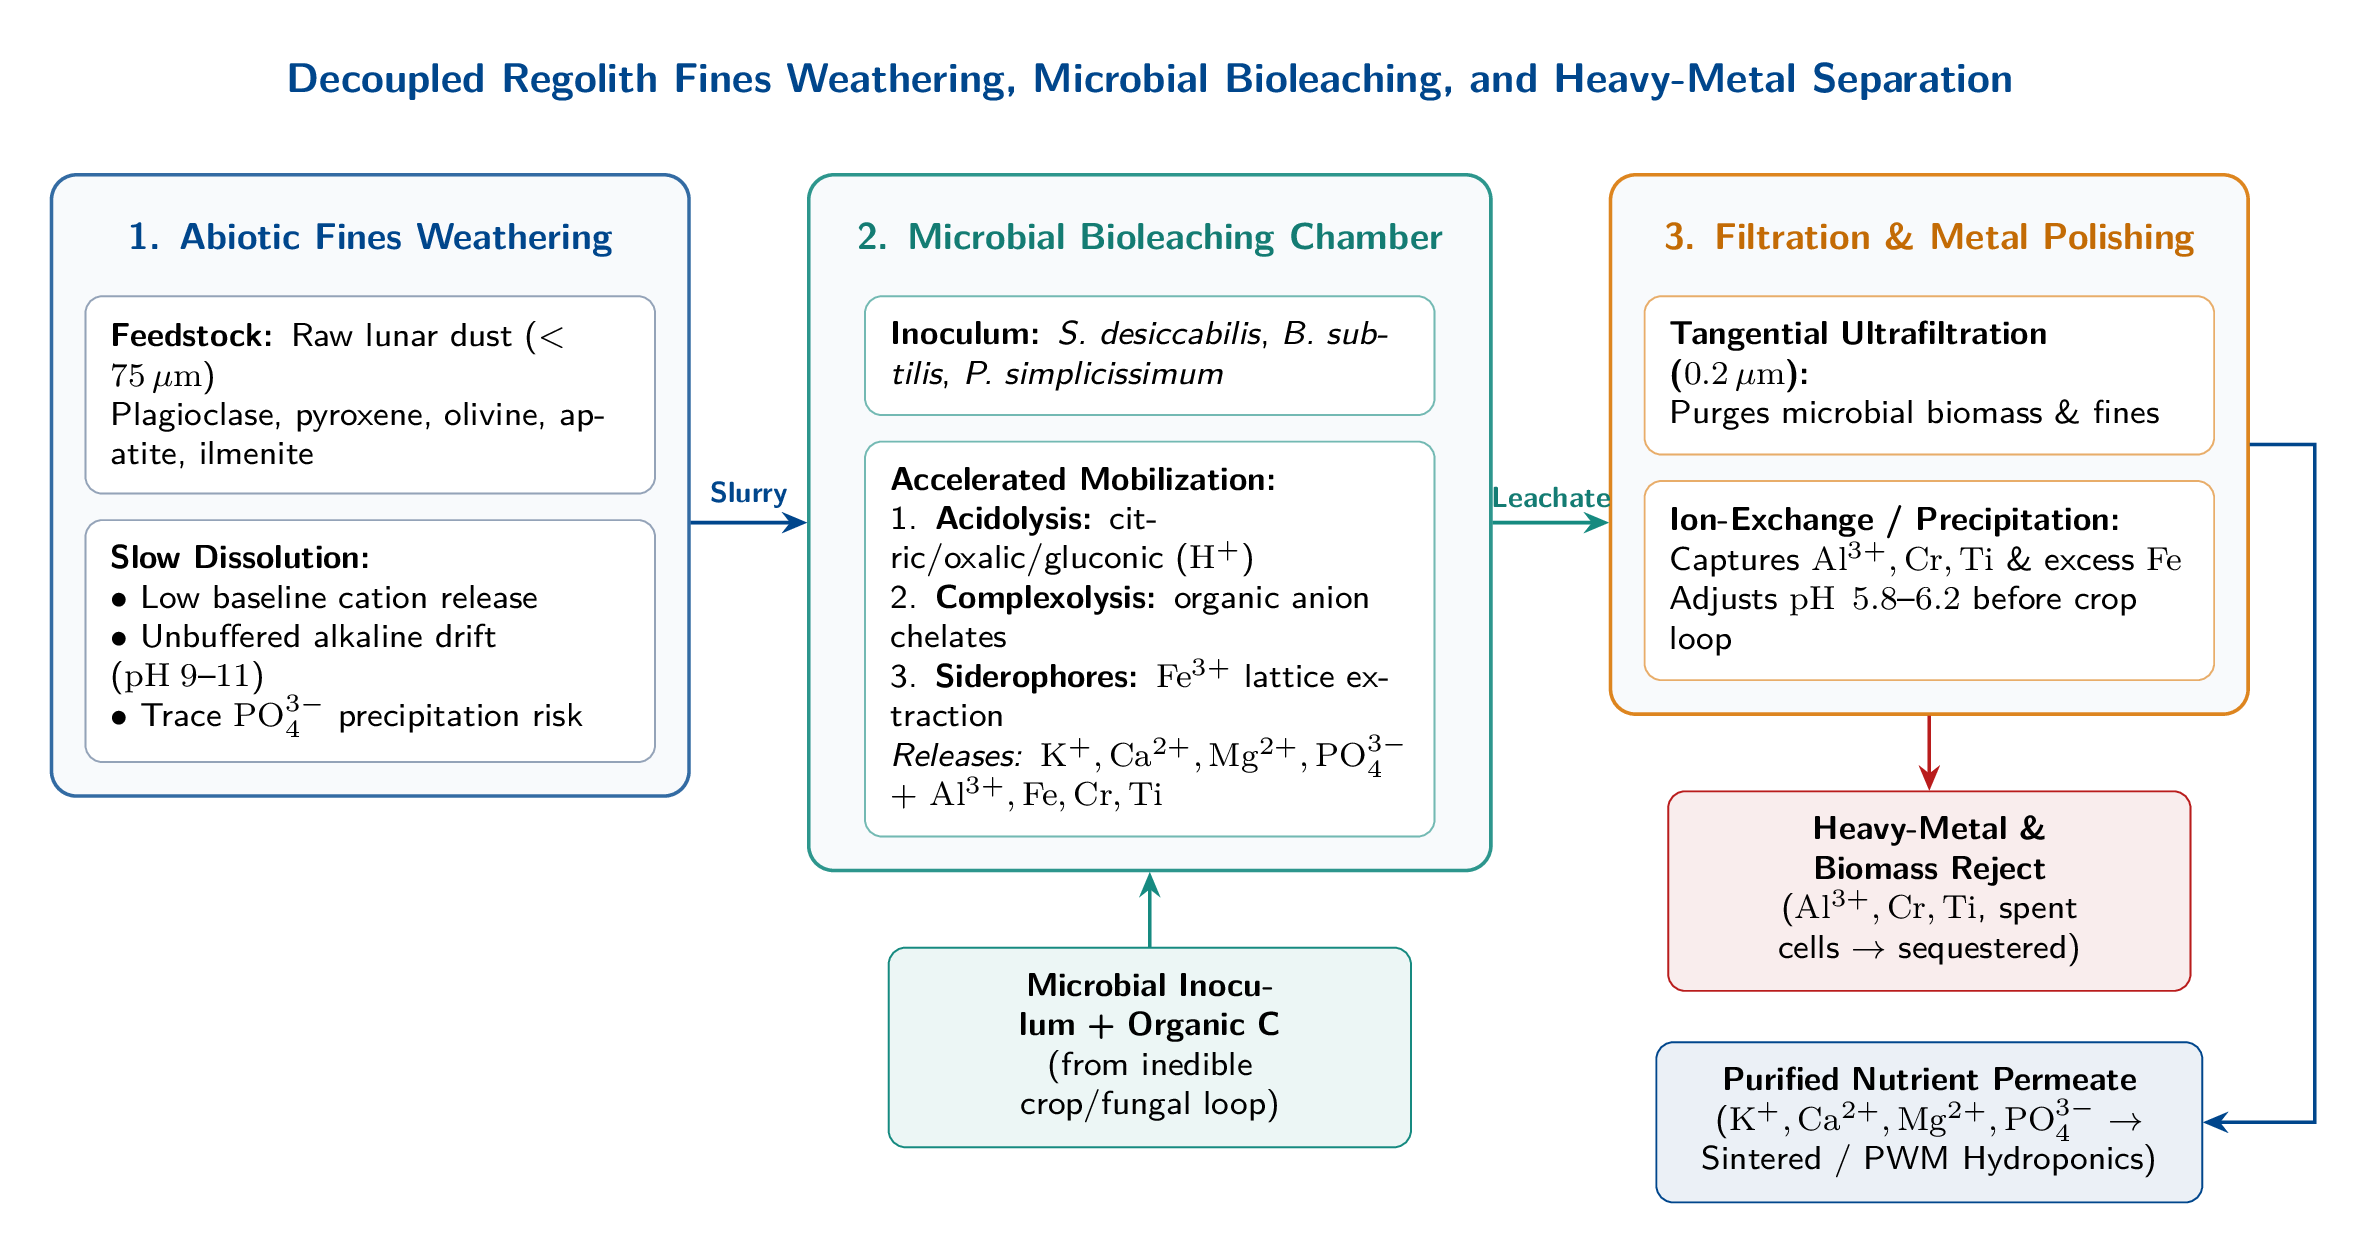
\includegraphics[width=\textwidth]{figures/fig5_bioweathering_chambers.png}
    \caption{\textbf{Decoupled regolith fines weathering, microbial bioleaching, and heavy-metal separation.} Raw lunar regolith fines ($<75\,\mu\mathrm{m}$) undergo baseline abiotic weathering before entering an external microbial bioleaching chamber inoculated with \textit{Sphingomonas desiccabilis}, \textit{Bacillus subtilis}, and \textit{Penicillium simplicissimum}\cite{cockell2018biorock,santomartino2024ecomine}. Organic acidolysis, complexolysis, and siderophore chelation accelerate nutrient mobilization ($\mathrm{K}^+, \mathrm{Ca}^{2+}, \mathrm{Mg}^{2+}, \mathrm{PO}_4^{3-}$) alongside dissolved metals ($\mathrm{Al}^{3+}, \mathrm{Fe}, \mathrm{Cr}, \mathrm{Ti}$). Subsequent $0.2\,\mu\mathrm{m}$ tangential ultrafiltration and ion-exchange polishing sequester heavy metals and spent biomass while returning purified, $\mathrm{pH}$-balanced ($5.8\text{--}6.2$) nutrient permeate to the sintered ceramic / PWM hydroponic loop\cite{ming1989lunar,weislogel2026pwm}.}
    \label{fig:bioweathering_chambers}
\end{figure}
